\chapter{Panorama des solutions industrielles}
\paragraph{}Nosu avons pu voir pourquoi il est préférable de privilégier le NoSQL au SQL pour la gestion des données géographiques, notamment au sein des \acrshort{SIG}. Pour compléter cela, nous allons faire un tour des solutions existantes que nous allons comparer selon des critères prédéfinis. Nous commencerons par un outil liés au relationnel pour avoir un regard sur ce qu’il existe. Nous passerons ensuite sur des SGBD NoSQL intégrant des modules liés aux SIG puis enfin SOLAP, un des outils les plus adaptés à l’analyse spatiale.

\section{Les critères de comparaison}

\paragraph{}Afin de pouvoir évaluer correctement chacune des solutions, il est primordial de définir des critères qui nous permettront de les comparer.

Nous avons pu voir pourquoi privilégier le NoSQL au SQL pour la gestion des données géographiques au sein des SIG. Pour compléter cela, nous aurons un tour d’aperçu des différentes solutions dans ce domaine. 

\subsubsection{Catégorie 1 : les caractéristiques du SGBD}
Ces critères, propres à chaque SGBD, seront étudiés à la fois dans la présentation des outils mais également dans l'application.
\begin{enumerate}
    \item \textbf{Le type} \\ Le \acrshort{SGBD} respecte-il les règles de Codd ou sort-il de ce paradigme ? \newline
    \item \textbf{Le schéma} \\ Le \acrshort{SGBD} permet-il un schéma fixe ou libre ? \newline
    \item \textbf{Le modèle} \\ Quel modèle est utilisé ? \newline
    \item \textbf{Le langage de requêtage} \\ Quel est le langage de requêtage principalement utilisé pour rechercher ou traiter des données ?
\end{enumerate}

\subsubsection{Catégorie 2 : les comparaisons dans l'implémentation de la base}
Ces critères permettant de comparer les bases de données seront étudiés dans l'application. Ils permettront d'évaluer l'occupation et l'implémentation des modèles.
\begin{enumerate}
    \item \textbf{Taille occupé par la base} \\ Quel est l'espace occupé ? \newline
    \item \textbf{Le nombre d'objets} \\ Combien d'objets sont contenus dans la base ? \newline
\end{enumerate}


\subsubsection{Catégorie 3 : l'exécution de la requête}
Ces critères permettant de comparer les bases de données seront étudiés dans l'application. Ils auront pour but de comparer les résultats fournis par les différents SGBD.
\begin{enumerate}
    \item \textbf{Temps d'exécution} \\ Quel temps a été utilisé pour réaliser la requête associée \newline
    \item \textbf{Nombre de résultats} \\ Nombre de tuples affichés \newline
    \item \textbf{Nombre d'objets manipulés} \\ Combien d'objets ont-ils été manipulés et lus pour répondre à la requête ?
\end{enumerate}


%Critères 
%standards : langage, modèle, type
%calculs : temps d'exécution, nb d'objets sollicités

\section{Des extensions SIG dans les SGBD relationnels}

\subsection{Les bases de données spatiales}

\paragraph{}Parmi toutes les informations qui circule dans le monde, 80\% ont un caractère spatial et nécessite des bases de données adaptées pour son traitement. L’architecture liée aux SIG a évolué au fur et à mesure des années : la première génération était centrée sur les outils avec un stockage dans les systèmes de fichiers, la deuxième était hybride mélangeant données SIG et attributaires et enfin la troisième et actuelle génération intègre données géométriques et attributaires sous un même schéma. Ceci facilite l’interaction entre les différents types de données. Différents types existent :
\begin{figure}[htp]
  \centering
  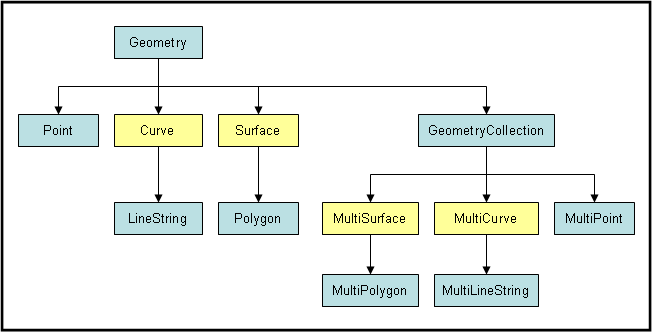
\includegraphics[width=140mm]{src_img/geometryhierarchy.png}
  \caption{Hiérarchie géométrique \supercite{hierarchygeo}}
  \label{fig:geometryHierarchie}
\end{figure}

\paragraph{}Comme le montre la figure \ref{fig:geometryHierarchie}, la géométrie d'un objet peut avoir plusieurs configurations : sous forme de point, de ligne ou de polygone. Cependant, chacun d'entre eux n'ont pas les mêmes propriétés, ils ne peuvent pas se retrouver dans une même table en suivant les standards relationnels. Nous aurons par exemple une table pour les limites de territoires (région, ville, quartier), une autre pour la topographie \footnote{topographie : relief d'un lieu} et une autre pour les données hydrographiques.

\paragraph{}Cette configuration par l'utilisation d'objets est l'un des principes mis en place par\newacronym{OGC}{OGC}{Open GeoSpatial Consortium} l’\acrfull{OGC} afin de permettre l'interopérabilité.


%\paragraph{}Comme nous pouvons le voir, les points, lignes et polygones caractérise l’aspect spatial des données mais n’ont pas le même standard au niveau SQL. En effet, chacun des objets ayant ses caractéristiques propres, elle ne peuvent être dans une même table : par exemple, une pour les limites d’une ville, une pour la topologie \footnote{Étude des déformations du sol}, une pour les données hydrographiques, etc. Cependant, \newacronym{OGC}{OGC}{Open GeoSpatial Consortium} l’\acrfull{OGC} a mis en place un certain nombre de principes pour permettre l’interopérabilité.

\subsection{Une large gamme de choix d'outils spatiaux relationnels}

\paragraph{}Dans les SIG intégrant des bases de données relationnelles, nous avons deux catégories.

\subsubsection{Les fonctions spatiales sur les SGBD traditionnels}
\paragraph{}Un certains nombre d'éditeurs de \acrlong{SGBD} ont mis en place au sein de leurs outils des extensions permettant à la fois de stocker et de réaliser des opérations sur des données spatiales. C'est le cas par exemple de MySQL, PostGreSQL et SQLite qui ont respectivement proposé MySQLSpatial, PostGreSQL et SpatiaLite. SAP HANA, Oracle Spatial, Microsft SQL Server ou DB2 sont également d'autres exemples de \acrshort{SGBD} relationnels qui offrent la possibilité de réaliser des requêtes spatiales.


%\paragraph{}Nous avons d'abord un certain nombre d'éditeurs de SGBD qui ont mis en place des extensions permettant de stocker et réaliser des opérations sur des données spatiales. C'est par exemple le cas de MySQL avec MySQL Spatial, PostGreSQL avec PostGIS et SQLite avec SpatiaLite. SAP HANA, Oracle Spatial, Microsft SQL Server ou DB2 sont d'autres exemples de systèmes de gestion de bases de données qui offrent la possibilité de réaliser des requêtes spatiales
\subsubsection{Les SIG intégrant les principes relationnels}
\paragraph{}La deuxième catégorie est celle des SIG intégrant eux-mêmes une lecture ou un stockage de données organisées de manière relationnelles. QGis intègre par exemple l'extension spatiale de PostGIS tout en permettant la gestion des données vectorielles. CARTO, un service de cartographie, aussi intégre la même extension.

%\paragraph{}Dans les SIG intégrant des bases de données relationnelles, nous avons deux catégories. Nous avons d'abord un certain nombre d'éditeurs de SGBD qui ont mis en place des extensions permettant de stocker et réaliser des opérations sur des données spatiales. C'est par exemple le cas de MySQL avec MySQL Spatial, PostGreSQL avec PostGIS et SQLite avec SpatiaLite. SAP HANA, Oracle Spatial, Microsft SQL Server ou DB2 sont d'autres exemples de systèmes de gestion de bases de données qui offrent la possibilité de réaliser des requêtes spatiales



\paragraph{}Pour notre étude, nous allons nous concentrer sur PostGIS, un des outils les plus présents dans ce domaine et nous allons donc le découvrir un peu plus en profondeur.

%\paragraph{}Un certain nombre d’éditeurs de SGBD relationnels ont mis en place des extensions spatiales parmi lesquels MySQL Spatial par MySQL, PostGIS par PostGreSQL. Il existe également des logiciels de SIG qui utilisent des bases de données relationnelles telles que nous les connaissons, c'est le cas de  Nous allons dans notre cas découvrir plus en profondeur PostGIS et ce qu’il permet.

\subsection{Zoom sur PostGIS}
\subsubsection{Présentation de l'outil}
\paragraph{}PostGIS, comme dit précédemment, est une module de PostGreSQL spécialement déjà à la gestion des données géographiques et géométriques. De ce fait, il respecte les standards SQL mais aussi les normes de l’OGC et ISO SQL/MM \cite{sqlmm} dédiés à ce type de données. Un des standards de l’\acrshort{OGC} utilisé par PostGIS est né avec \newacronym{SFS4SQL}{SFS4SQL}{Simple Features Specification for SQL}le \gls{SFS4SQL} et la représentation des objets géométriques avec le format de données \newacronym{WKT}{WKT}{Well Know Text} \gls{WKT} \cite{coursPostGIS} et son dérivé binaire : \newacronym{WKB}{WKB}{Well Know Binary} le \gls{WKB}. En 2000 est également créé  \newacronym{GML}{GML}{Geography Markup Language} le \gls{GML} pour faciliter l’interopérabilité des données mais également \newacronym{KML}{KML}{Keyhole Markup Language} le \gls{KML}, spécialement utilisé par Google Earth.

\subsubsection{Ses composants}
\paragraph{}Pour atteindre ses objectifs, PostGIS s’est servis des fonctionnalités de PostGreSQL auxquelles se sont ajoutés différents couplages : avec Proj4 pour les projections géographiques, GEOS\footnote{GEOS : une librairie Java pour les objets géométriques} pour les opérateurs spatiaux et \newacronym{GDAL}{GDAL}{Geospatial Data Abstraction Library} \gls{GDAL} pour les fonctionnalités raster. En plus de gérer les types de données spatiales et des opérateurs, PostGIS propose plusieurs types d'index : B-tree, R-tree, Hash et GiST.

\newglossaryentry{ldd}
{
    name=définition de données,
    description={les fonctions de manipulation des tables : Create, Alter, Drop}
}
\newglossaryentry{lmd}
{
    name=manipulation de données,
    description={les fonctions permettant d'agir sur les données : Insert, Update, Delete, Select}
}
\paragraph{}En plus des fonctions de \gls{ldd} et de \gls{lmd} LMD , PostGIS dispose d’un certain nombre de fonctions pour les différents objets :
\begin{itemize}[label=\textbullet]
    \item pour tous : retourner les objets sous format WKT, GML
    \item pour les points : récupérer ses coordonnées X et Y
    \item pour les lignes : avoir la distance, le point de départ et d’arrivée
    \item pour les polygones : obtenir l’aire, le périmètre, les contours
\end{itemize}
\paragraph{}Sont également présentes des fonctions pour calculer les distances entre objets, s’ils se collent ou se chevauchent, etc.

\subsubsection{La vérification des critères}
\paragraph{}A partir des informations sur le \acrshort{SGBD}, il est possible de compléter les critères énoncés au départ.
\begin{table}[h!]
    \centering
	\begin{tabular}{|p{5cm}|p{7cm}|} 
  	\hline
  	\textbf{Critère} & \textbf{Valeur} \\
  	\hline
  	1.1 : respect principes Codd & Oui, il possède des relations \\
  	\hline
  	1.2 : schéma utilisé & Fixe \\
  	\hline
  	1.3 : modèle utilisé & Relationnel \\
  	\hline
  	1.4 : langage de requêtage & SQL \\
  	\hline
	\end{tabular}
    \caption{Table des critères concernant PostGIS}
    \label{tab:critere-postgis}
\end{table}

\section{Développement des SIG avec le NoSQL}
\paragraph{}Dans la partie précédente, nous avons pu voir que les systèmes de gestion de bases de données orientés NoSQL gèrent plus facilement les larges quantités de données. Contrairement aux bases de données relationnelles limitées à une machine, le NoSQL dispose d’une architecture répartie lui conférant une plus grande puissance de calcul. Nous verrons l’exemple de MongoDB.

\subsection{Présentation de MongoDB}

MongoDB est un système de gestion de base de données orienté documents développé par MongoDB Inc. et publié pour la première fois en 2009. Il permet de manipuler des objets structurés au format BSON sans schéma prédéfini de données. Ces objets sont des documents enregistrés dans des collections. De ce fait, une collection peut avoir deux objets avec des champs totalement différents. Dans un document, des champs peuvent être ajoutés, supprimés, modifiés et renommés à tout moment. Il est également possible d’imbriquer des documents. Aussi, il n’utilise pas le SQL comme les SGBD relationnels mais soit des instructions en ligne de commande, soit via des langages de programmation comme le C, le PHP ou le Dart.

\subsection{Pourquoi son format est adapté aux SIG}
Comme énoncé juste au-dessus, MongoDB est de type document et possède un format BSON dérivé du JSON. Cette configuration lui permet de contenir des données sans schéma précis. Pour pallier à certains besoins, un format de fichier, le GeoJSON, a été développé par des développeurs et est aujourd’hui utilisé par OpenStreetMap ou Python. Par ailleurs, MongoDB a l’avantage de permettre de manipuler à la fois vecteur et raster alors que Cassandra \cite{mongovecteur} permet uniquement la manipulation de raster.
En voici un exemple :
\begin{verbatim}
{
  "type": "Feature",
  "geometry": {
    "type": "Point",
    "coordinates": [125.6, 10.1]
  },
  "properties": {
    "name": "Dinagat Islands"
  }
}
\end{verbatim}



\paragraph{}Il donne également plus de possibilités d’index. Comme d’autres outils, il utilise les arbres B et Quadtree mais il utilise également 2d et 2dsphere\cite{2dsphere}. Ce dernier est particulièrement important du fait qu’il calcule sur une surface similaire à la Terre. Également face à l’augmentation de la quantité de données, MongoDB permet d’avoir des meilleures vitesses d’exécution.

\subsection{Critères de comparaison}

\paragraph{}A partir des informations sur le \acrshort{SGBD}, il est possible de compléter les critères énoncés au départ.
\begin{table}[h!]
    \centering
	\begin{tabular}{|p{5cm}|p{7cm}|} 
  	\hline
  	\textbf{Critère} & \textbf{Valeur} \\
  	
  	\hline
  	1.1 : respect principes Codd & Non, il respecte un autre paradigme (NoSQL) \\
  	\hline
  	1.2 : schéma utilisé & Libre \\
  	\hline
  	1.3 : modèle utilisé & Document \\
  	\hline
  	1.4 : langage de requêtage & Langage propre \\
  	\hline
	\end{tabular}
    \caption{Table des critères concernant MongoDB}
    \label{tab:critere-mongo}
\end{table}


\section{SOLAP}

\paragraph{}L’outil SOLAP (Spatial OnLine Analytical Processing) a été proposé en 1995 par Yves Bédard de l’Université de Laval au Québec. Il le définit comme une «\textit{une plate-forme visuelle supportant l'exploration et l'analyse spatio-temporelle faciles et rapides des données}» suivant une approche multidimensionnelle. Cette dernière, à plusieurs niveaux d'agrégation permet à la fois un affichage cartographique, tabulaire ou statistique \cite{defsolap}. Il permet donc de traiter les données, les analyser avec OLAP et en ressortir une visualisation cartographique. D’abord réservés aux bases de données relationnelles, les outils de traitement analytique en ligne se sont peu à peu ouverts aux structures pas ou semi-structurée du NoSQL.

\begin{figure}[htp]
  \centering
  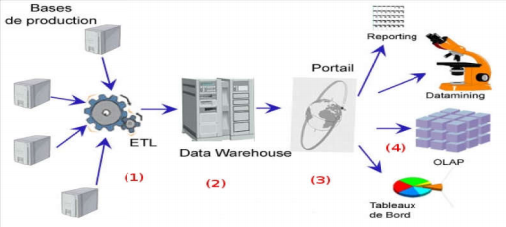
\includegraphics[width=95mm]{src_img/fonctionnementOLAP.png}
  \caption{Fonctionnement OLAP \supercite{fonctionnementSOLAP}}
  \label{fig:olap}
\end{figure}
\paragraph{}Comme indiqué précédemment, les données NoSQL sont hétérogènes et c’est particulièrement le cas avec les données géographiques qui comprennent des données géométriques (lignes, points, polygones) mais également des données associées. Cette structure amène des besoins d’analyse\cite{solap} plus approfondies.

\begin{table}[h!]
    \centering
	\begin{tabular}{|p{5cm}|p{7cm}|} 
  	\hline
  	\textbf{Critère} & \textbf{Valeur} \\
  	\hline
  	1.1 : respect principes Codd & Oui, il respecte les relations \\
  	\hline
  	1.2 : schéma utilisé & Fixe \\
  	\hline
  	1.3 : modèle & Relationnel \\
  	\hline
  	1.4 : langage de requêtage & SQL avec quelques autres fonctions (ROLLUP, GROUPING, etc)  \\
  	\hline
	\end{tabular}
    \caption{Table des critères concernant SOLAP}
    \label{tab:critere-solap}
\end{table}

\section{Les SIG as a Service, une offre en expansion}
\paragraph{}Depuis quelques années, le cloud computing avec ses paradigmes s'est imposé dans la distribution de logiciels et a permis à de nouvelles plateformes de se développer. Les entreprises développant les SIG ont donc dû s'adapter pour proposer des architectures plus flexibles et simples d'utilisation.

\paragraph{}L'augmentation des plateformes géospatiales dans le cloud a entraîné un changement de comportement vis-à-vis du travail des données spatiales. Parmi les principaux avantages, il y a le partage d'informations facilité, la spécialisation de certains outils, la simplicité obtenue dans l'utilisation, la baisse des coûts et le potentiel de croissance.

\paragraph{}Le Software as a Service (SaaS) permet aux utilisateurs d'utiliser une solution installée sur des serveurs distants et non sur la machine de ce dernier. Cela passe essentiellement par un service en ligne avec abonnement. Parmi les SIG qui utilisent le SaaS, nous avons ArcGIS, développé par ESRI. Cet outil permet le reporting et la création de tableaux de bord métier à partir de cartographie et d'analyse spatiale. D'autres outils comme CARTO, déjà cité auparavant et MapBox, fournisseur de cartes personnalisées utilisent également cette architecture.

\paragraph{}Une autre catégorie de plateformes est le PaaS, le Platform as a Service, où le fournisseur cloud maintient l'infrastructure et le matériel et le client maintient pour sa part l'application. ArcGis founit aussi cet architecture en terme de solution tout comme les API de Google Maps ou Geocode Dataflow de Microsoft.

\paragraph{}Le DaaS, Data as a Service, est le dernier type d'architecture utilisé dans les SIG. Il permet à l'utilisateur d'être uniquement facturé par le fournisseur pour les données qu'il souhaite utiliser. Cela passe par la délégation du stockage et de la gestion des données. Cela est par exemple utilisé par les outils de cartographie comme Google Maps ou OpenStreetMap.


\section{Synthèse et critique}

Nous avons pu dans cette partie comparer l'exemple en terme de gestion des SIG. D'un côté, PostGIS utilise les fonctions traditionnelles des SGBD relationnels pour gérer les objets géométriques. Il se base sur de nombreux standards à la fois ISO et OGC pour permettre une meilleure interopérabilité. De l'autre, nous avons MongoDB qui grâce à sa gestion des documents permet une gestion optimisée des documents comme l'est le GeoJSON. Egalement, face aux besoins de plus en plus importants d'analyses multidimensionnelles, SOLAP permet d'intégrer la dimension spatiale aux outils traditionnels. Le développement du cloud computing a également apporté diverses possibilités.

\paragraph{}De petits projets utilisant des données géographiques peuvent utiliser des systèmes de gestion de données relationnels comme PostGreSQL et son module PostGIS. Cependant, avec l'accroissement continu de la quantité de données échangées dans le monde, dont 80\% représentent des données spatiales, il s'avère plus qu'important d'utiliser des architectures de bases de données adéquates et les bases de données telles que MongoDB peuvent représenter une solution. Si une analyse multidimensionnelle est nécessaire, il est également possible de se tourner vers SOLAP.